\section{Implementation}
The implementation of distance measurement has been done by using the method of time of flight. There are two stations each mounted with transmitter and receiver module respectively. The transmitter module contains a ultrasonic transmitter and receiver section contains a ultrasonic receiver and we measure the time of flight of the sound signal that originates from the transmitter station ending up at the receiver station.

\subsection{Synchronization}
Synchronization is the most crucial part of the whole process of distance measurement. The receiver must exactly know when the transmitter is going to send the incoming signal in order to have the prior knowledge to start the time within it. It is not possible to know when exactly the transmitter will send the incoming signal but we can achieve somewhat close approximation by the use of light transmitter and receiver. 

The speed of light is approximately $3\times 10^8 m/s$. If we set up transmitter such that the transmitter station sends a pulse of light and sound at the same time, the light pulse reaches the receiver at no time compared to the sound pulse due to the massive difference of speed of each of these.

\subsubsection{Calculation}
If the distance between light transmitter and receiver is $x$, then the time taken by light to reach the receiver station is 
\begin{equation}
	t_l = \frac{x}{c}
\end{equation}
Where $t_l$ is the time taken by light to reach the receiver station. Similarly time taken by sound to reach the receiver station is given by the relation.

\begin{equation}
	t_s = \frac{x}{v_s}
\end{equation}
where $v_s$ is the speed of sound.

Now as soon as the receiver station detects the light signal, we start the timer and stop the timer as soon as it detects the sound signal.
The time recorded by the receiver station will thus be 
\begin{equation} \label{eq:deltaT}
	\Delta t = x\left( \frac{1}{v_s}- \frac{1}{c}\right)
\end{equation}
Since $c >> v_s$ $\Delta t \approx \frac{x}{v_s}$. 
The error committed in the process is 
\begin{equation} 
	\epsilon = x\left( \frac{1}{v_s}- \frac{1}{c}\right) - \frac{x}{v_s}
\end{equation}

Which gives us the error percentage of 
\begin{eqnarray*}
	Error \% & =& \frac{\epsilon}{t_s}\times 100\%\\
	{}& = & \frac{v_s}{c} \times 100 \%\\
	{}& \approx & 0.0001\% 
\end{eqnarray*}

We thus place at the transmitter side a \gls{irled} and a ultrasonic signal transmitter. At the receiver we place ultrasonic receiver and a TSOP. The TSOP detects the light signal.

\begin{figure}
	\centering
	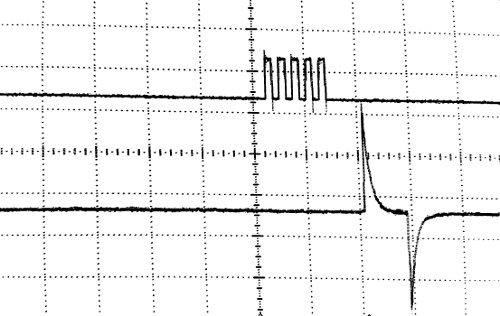
\includegraphics[width=120mm]{Images/DetectionByTSOP.jpg}
	\caption{TSOP response to detected IR signal by IRLED}
	\label{fig:DetectionByTSOP}
\end{figure} 
In Figure.\ref{fig:DetectionByTSOP} the upper waveform is the signal fed to the \gls{irled} transmitter and the lower waveform is the response of TSOP circuitory to the detected signal.

\subsection{Ultrasound transmission}
The ultrasonic transmitter typically works at a frequency of $40kHz$. So we generate the required signal using  a microcontroller. The microcontroller generates the required signal by pulling a particular pin at high and low at calculated intervals. Following piece of code is written in C for ATmega8 to generate 40kHz signal at a particular pin.

\begin{lstlisting}
void DriveIRLED()
{
	int Peaks = 5;
	int i = 0;
	for(;i< Peaks*2; i++) {
		TOGGLE(PORTC,PC5);
		_delay_us(4);
	}
}
\end{lstlisting}

\begin{figure}
	\centering
	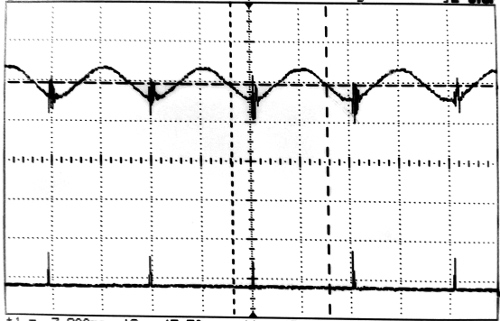
\includegraphics[width=120mm]{Images/UltrasonicTransception.jpg}
	\caption{Signal Transmission and Reception by Ultrasonic pair}
	\label{fig:UltrasonicTransception}
\end{figure}
In Figure.\ref{fig:UltrasonicTransception} the lower signal with regular spikes is the signal applied to Ultrasonic transmitter. Each spike (contracted in time) is a brust of square wave pulses shown in Figure.\ref{fig:SignalBrust}. The interval of each burst is $2ms$. The upper signal in Figure.\ref{fig:UltrasonicTransception} is the response of Ultrasonic receiver to the obtained signal. There are clear spikes  detected at exactly the interval sent by the transmitter.
\begin{figure}
	\centering
	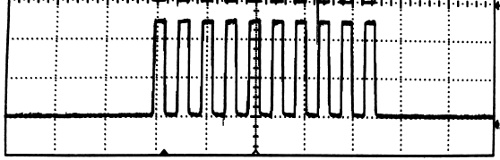
\includegraphics[width=120mm]{Images/SignalBrust.jpg}
	\caption{40kHz Signal Brust applied at ultrasonic transmitter}
	\label{fig:SignalBrust}
\end{figure}
 
Since the received signal is noisy and very low power, it requires to be amplified and filtered for the required frequency.
\subsection{Signal Amplification}

The received sound signal is converted
by into electrical signal by ultrasonic receiver. Since the sound undergoes massive attenuation in air, the received signal is pretty low in voltage and needs to be amplified in order to use it for distance measurement. 

An amplifier is an electronic device that increases the power of a signal. An operational amplifier ("op-amp") is a \gls{dc} coupled high-gain electronic voltage amplifier with a differential input and, usually, a single-ended output. In the configuration as shown in Figure.\ref{fig:InvertingAmplifier}, an op-amp produces a output potential that is typically hundreds of thousands of times larger than the potential difference between its input terminals. 

\begin{figure}[h]
	\centering
	\begin{circuitikz}[scale=0.75,transform shape] \draw
		(4,-.5) node[op amp](opamp1) {}
		
		(1,0) node[anchor=east] {$V_{in}$}	
		to [R=$R_g$,o-*] (opamp1.-)
		to [short](2.8,1)
		to [R=$R_f$] (5.2,1)
		to [short,-*] (opamp1.out)
		
		(opamp1.out) to [short,-o] (6.2,-0.5)
		node[anchor=west] {$V_{out}$}
		(opamp1.+) to [short] ($(opamp1.+)+(0,-1)$)node [ground] {}
		;
		
	\end{circuitikz}
	\caption{A negative feedback inverting Amplifier}
	\label{fig:InvertingAmplifier}
\end{figure}


The output voltage of this operational amplifier closed loop negative feedback is given by :-
\begin{equation}
	V_{out} = -\frac{R_f}{Rg}V_{in}
\end{equation} 


Where,\\ $R_f$ is feedback resistor \\$R_g$ is input resistance. \\$V_{in}$ is input voltage, \\$V_{out}$ is output voltage. 

The gain of the amplifier is controlled by two resistors, $R_f$ and $R_g$. The gain is the ratio of the feedback resistor to the input resistor. However, the opamp we used,i.e. UA741 has a maximum practical gain of 2.5 dB only. Since the electrical signal produced by the ultrasonic receiver is pretty low in voltage, it needs to be amplified by using a two-stage amplifier. The circuit diagram for two stage amplifer is as shown in Figure.\ref{fig:TwoStageAmplifier}, where the output of one amplifier is fed as an input to the exactly same another amplifier circuit.

\begin{figure}[h]
	\centering
	\begin{circuitikz}[scale=0.75,transform shape] \draw
		(4,-.5) node[op amp](opamp1) {}
		(9,-.5) node[op amp](opamp2) {}
		
		(1,0) node[anchor=east] {$V_{in}$}	
		to [R=$R_1$,o-*] (opamp1.-)
		to [short](2.8,1)
		to [R=$R_2$] (5.2,1)
		to [short,-*] (opamp1.out)
		
		(opamp1.out) to [R=$R_3$] (7.8,-0.5)
		to [short,-*] (opamp2.-)
		to [short] (7.8,1)
		to [R=$R_4$] (10.2,1)
		to [short,-*] (opamp2.out)
		
		(opamp2.out) to [short,-o] (12,-0.5)
		node[anchor=west] {$V_{out}$}
		(opamp1.+) to [short] ($(opamp1.+)+(0,-1)$)node [ground] {}		
		(opamp2.+) to [short] ($(opamp2.+)+(0,-1)$)node [ground] {}
		;
		
	\end{circuitikz}
	\caption{Two Stage Amplifier}
	\label{fig:TwoStageAmplifier}
\end{figure}

	
	
Thus the low voltage signal received through the receiver of ultrasonic senser was amplified using operational amplifier with negative feedback. The values of the component of this operational amplifier is calculated so that we could get the required signal strength. The amplified signal is now fed into the input of tone decoder circuit.

\subsection{Signal Filtering}

The transducer will pick up most sounds within a fairly wide range. Thus ultrasonic signal received by the receiver not just contain the 40kHz required signal. It also comprises of some other noise signals. To make sure the system only picks up the ultrasound signal that was transmitted, we need to lock the receiver onto a frequency of 40kHz. 

For this, we have used IL567 Tone Decoder \gls{ic}. This tone decoder is a general purpose tone decoder which looks for a close match between the frequency of incoming signal and of its internal oscillator. The frequency of it's internal oscillator can be controlled by adjusting the values of capacitor and resistor between Pin 5 and Pin 6 of the \gls{ic}. The frequency of internal oscillator is given by the expression :\cite{Yichao}

\begin{equation}
	f=\frac{1}{1.1*R*C}
\end{equation}
where,
R = Resistor placed between Pin 5 and Pin 6
C = capacitor placed at Pin 6
\begin{figure}[h]
	\centering
	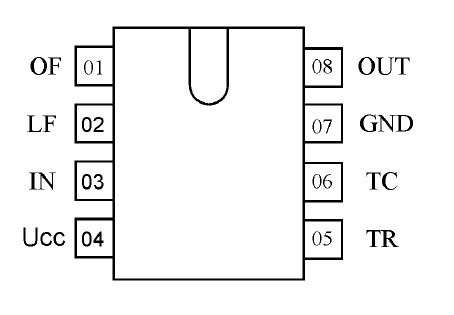
\includegraphics[scale=0.5]{Images/IL567PinOut.jpg}
	\caption{IL567 Pin Out}
	\label{fig:PinOut}
\end{figure}

\begin{table}[h!]
	\centering
	\begin{tabular}{|c|c|c|}
		\hline 
		\bf{Pin Number} & \bf{Symbol} & \bf{Description} \\ 
		\hline 
		01 & OF & FIlter output \\	
		02 & LF & Loop Filter \\
		03 & IN & Frequency Input \\	  
		04 & $U_{cc}$ & Supply Voltage \\	  
		05 & TR & Timing Resistor \\	  
		06 & TC & Timing Capacitor \\	  
		07 & GND & Common Pin(Ground) \\	  
		08 & OUT & Output \\ 
		\hline 
	\end{tabular} 
	\caption{Pin Description of IL567 \gls{ic}\cite{ToneDecoder}}
\end{table}

This IC sets it's output(Pin 8) to low when the frequency of incoming signal matches the frequency of internal oscillator. When there is incoming signal of other frequencies or there is no signal at all, the output(Pin 8) remains high. 
We used a capacitor of 0.01$\mu$ F. In order to lock the frequency of internal oscillator at 40kHz, we need a resistor of approximately 2.272 K$\Omega$ . Now since exactly this value resistor was not available, we used a potentiometer of 10K instead of this resistor. 

\subsection{Fixing the frequency of internal oscillator}

To make sure that the tone decoder recognizes 40kHz signal and sets it output to low only on the arrival of 40kHz signal, the frequency of it's internal oscillator needs to be fixed at 40kHz. Since we do not have exactly 2.272K$\Omega$ resistor available, we use a potentiometer to adjust the frequency of internal oscillator.

We fed a 40kHz sinusoidal signal to the input of the IL567 from function generator. Since the output of the IC is high when the frequency of incoming signal does not match the frequency of internal oscillator or also when there is no signal whatsoever, initially the output of this IC was high. Now the potentiometer was adjusted until the output of the IC was low. Thus, the frequency of internal oscillator of the IL567 was finalised to 40kHz.
\begin{figure}[h]
	\centering
	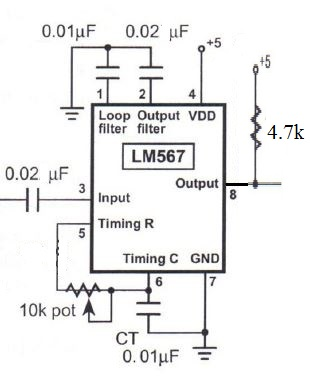
\includegraphics[scale=0.7]{Images/ToneDecoder.jpg}
	\caption{Circuit Diagram for Tone Decoding}
	\label{fig:CircuitDiagramForToneDecoding}
\end{figure}

\subsection{Detection of incoming signal}
The ultrasonic receiver receives the 40kHz signal transmitted from the transmitter. This signal is amplified using a two stage operational amplifier. The output of the amplifier circuit is fed as an input to the IL567. Now, as soon as the output of the IL567 goes low, we can know that the incoming signal is the transmitted signal with frequency of 40kHz. Thus, this can operate as a bandpass filter at 40kHz.

The output pin (Pin 8) on the LM567 Tone Decoder is connected to an input configured I/O pin on the microcontroller so that it is able to detect signals from the LM567 Tone Decoder. When the output pin (Pin 8) on the LM567 Tone Decoder is pulled low, the microcontroller knows that an ultrasonic signal has been received, and it stops running the counter and calculates the travel time of the signal.

\subsection{Distance Calculation}
Now equipped with all these stages we are finally able to calculate the distance between the transmitter and receiver station. Since we have the time recorded, we can use the time recorded using Equation.\ref{eq:deltaT} to calculate the original distance. Let the time recorded by the receiver station be $T_r$. Then we can use this recorded time to calculate distance as
\begin{eqnarray*}
	d &=& T_r \times v_s\\
	{}&=&\Delta t \times v_s\\
	{}&\approx&\frac{x}{v_s} \times v_s\\
	{}& = & x
\end{eqnarray*}
Thus we can find the actual distance $x$ by this process.

\subsection{Circuit Realization}
We have made the transmitter circuit which 

\begin{figure}
	\centering
	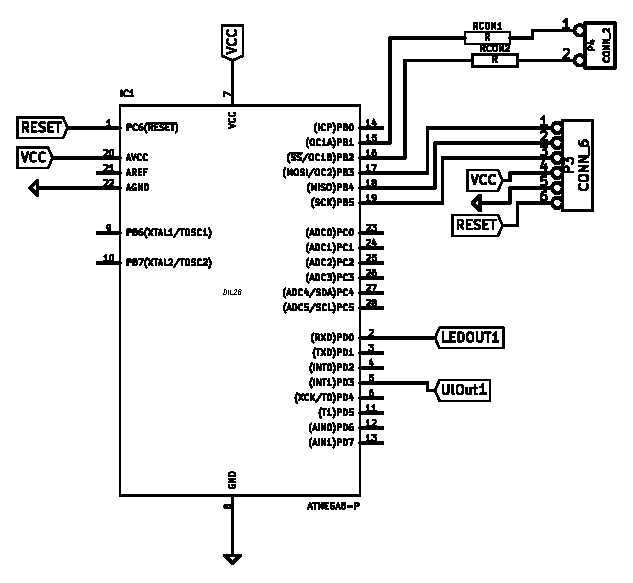
\includegraphics{Images/PWMGenerator.eps}
	\caption{PWM Signal Generator}
	\label{fig:PWMGenerator}
\end{figure}

The generated \gls{pwm} signal is fed to the Ultrasonic Transmitter, but signal sinking causes the signal to die out in the ultrasonic transmitter. So we have used a transistor to decouple the circuit from the ultrasonic transmitter. Figure.\ref{fig:Transmitter} shows the Ultrasonic transmitter attached to the output pin of \gls{pwm} generator in Atmega8/
\begin{figure}
	\centering
	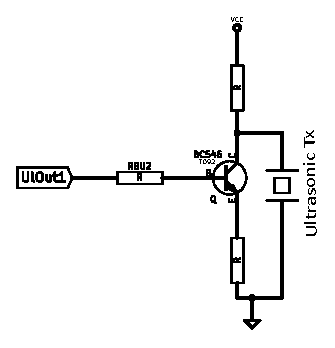
\includegraphics{Images/Transmitter.eps}
	\caption{Ultrasonic transmitter driven by \gls{pwm}}
	\label{fig:Transmitter}
\end{figure}

Also for synchronization process \gls{irled} is also driven by the microcontroller. Figure.\ref{fig:IRLEDCircuit} shows the \gls{irled} attached to the \gls{pwm} generator.

\begin{figure}
	\centering
	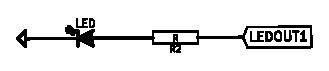
\includegraphics{Images/IRLEDCircuit.eps}
	\caption{\gls{irled} driven by \gls{pwm}}
	\label{fig:IRLEDCircuit}
\end{figure}

Finally a \gls{pcb} is made for the transmitter which is shown in Figure.\ref{fig:TransmitterPCB}.

\begin{figure}
	\centering
	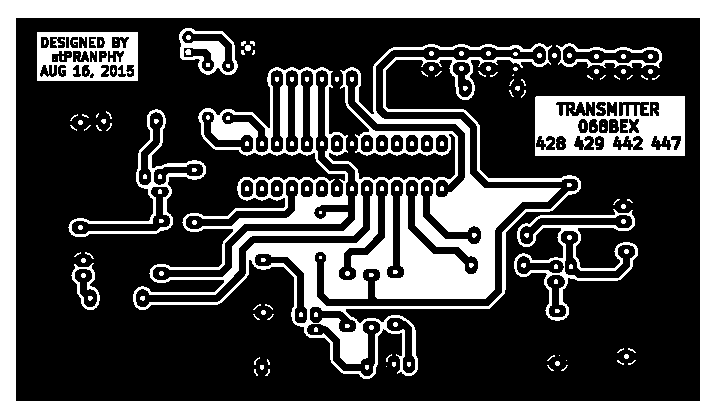
\includegraphics{Images/TransmitterPCB.eps}
	\caption{\gls{pcb} of the transmitter section}
	\label{fig:TransmitterPCB}
\end{figure}

